\documentclass[aspectratio=169,11pt]{beamer}
\usepackage{beamerucad}
\usepackage{listings}
\definecolor{ckw}{HTML}{2563AB}\definecolor{cst}{HTML}{2E8B57}\definecolor{ccm}{HTML}{8A8F98}
\lstdefinestyle{jv}{language=Java,basicstyle=\ttfamily\footnotesize,
 keywordstyle=\color{ckw}\bfseries,stringstyle=\color{cst},commentstyle=\color{ccm}\itshape,
 showstringspaces=false,columns=fullflexible,keepspaces=true,
 backgroundcolor=\color{ucadband!8},frame=leftline,framerule=2.5pt,rulecolor=\color{ucadband},
 xleftmargin=8pt,aboveskip=3pt,belowskip=1pt,basewidth=0.5em}
\lstset{style=jv}
\title{Architectures Logicielles — Séance 4}
\subtitle{L'extraction : un module quitte le monolithe et devient un microservice}
\author{Dr. El Hadji Bassirou TOURÉ}
\institute{Département de Mathématiques et Informatique\\ Faculté des Sciences et Techniques\\ Université Cheikh Anta Diop de Dakar}
\date{}
\setucadfoot{Architectures Logicielles --- Séance 4 \quad\textbullet\quad Dr. El Hadji Bassirou TOURÉ --- DMI/FST/UCAD}
\graphicspath{{figs/}}
\begin{document}

\begin{frame}[plain,noframenumbering]\titlepage\end{frame}

\begin{frame}{Objectifs de la séance}
\begin{ucaddef}[Contenu]
{\small Le module \texttt{livraison} quitte le monolithe : il devient \textbf{livraison-service}, un microservice \textbf{FastAPI} en Python, extrait selon le pattern \textbf{Strangler Fig}. L'appel qui traversait la JVM traverse désormais \textbf{le réseau} — avec ses promesses (déploiement indépendant, écosystème Python) et ses dangers, que nous éprouverons en \textbf{provoquant une panne}. Au passage : \textbf{docker compose} orchestre nos quatre conteneurs, et une \textbf{carte Leaflet de Dakar} suit le livreur en temps réel.}
\end{ucaddef}
\begin{itemize}\small
  \item Savoir répondre à la vraie question : \emph{quand} un microservice mérite-t-il son coût ?
  \item Extraire sans interrompre : le pattern \textbf{Strangler Fig}, rendu possible par le modulith.
  \item Mesurer ce que change un \textbf{appel réseau} — latence, pannes, et la troisième issue.
  \item Orchestrer avec \textbf{docker compose} ; visualiser avec \textbf{Leaflet} — zéro clé API.
\end{itemize}
\end{frame}

% #####################################################################
\section{Pourquoi extraire ?}

\begin{frame}{La demande de la direction}
\begin{ucadex}[Le scénario]
{\small La direction veut faire évoluer le calcul d'itinéraires : optimisation, trafic, géospatial — le terrain de \textbf{l'écosystème Python} (geopandas, OR-Tools). Et déployer ces évolutions \textbf{chaque semaine, sans redéployer} SénResto.}
\end{ucadex}
\begin{itemize}\small
  \item Deux besoins qu'un monolithe, même modulaire, ne peut pas offrir : \textbf{une autre technologie} pour un module, et \textbf{un déploiement indépendant} — les deux bonnes raisons classiques, avec une troisième : le \textbf{dimensionnement} indépendant.
\end{itemize}
\begin{ucadpiege}[Les mauvaises raisons existent aussi]
{\footnotesize « C'est moderne », « Netflix le fait », « le CV »... Un microservice injustifié, c'est tout le coût du réseau sans aucun bénéfice. La charge de la preuve incombe \emph{toujours} à l'extraction.}
\end{ucadpiege}
\end{frame}

\begin{frame}{Pourquoi livraison — et pas un autre ?}
{\small Les critères d'un bon candidat à l'extraction, appliqués à nos modules :}
\vskip2pt
{\small\begin{tabular}{p{0.30\linewidth}p{0.14\linewidth}p{0.40\linewidth}}
\toprule
\textbf{Critère} & \textbf{livraison} & \textbf{contre-exemple}\\
\midrule
Frontière déjà nette & oui (Lab 3) & —\\
API étroite & 3 opérations & \texttt{commandes} : au c\oe ur de tout\\
Données peu partagées & les livreurs & \texttt{catalogue} : lu par tous\\
Raison technologique & Python géo & \texttt{notifications} : aucune\\
Raison de déploiement & évolutions fréquentes & \texttt{partage} : jamais\\
\bottomrule
\end{tabular}}
\vskip4pt
\begin{ucadret}[À retenir]
{\small On n'extrait pas « les modules » : on extrait \textbf{un} module, celui dont l'extraction a une raison d'être. Les autres restent — et c'est très bien ainsi. Votre ADR n\textsuperscript{o}4 devra défendre ce choix \emph{et} les non-choix.}
\end{ucadret}
\end{frame}

% #####################################################################
\section{Le Strangler Fig}

\begin{frame}{L'idée simple : déménager sans fermer}
\begin{ucadex}[La boutique du coin]
{\small Un boutiquier veut plus grand. Il ne ferme pas pour tout casser :
il \textbf{construit la nouvelle boutique juste à côté}, puis déplace
\textbf{un rayon à la fois}. Les clients achètent \textbf{tous les jours,
sans rien remarquer}. Un rayon pose problème ? Il le \textbf{ramène}.
L'ancienne est vide ? Il la ferme.}
\end{ucadex}
{\small Dans notre lab, mot pour mot :}
\begin{itemize}\small
  \item la nouvelle boutique $=$ \texttt{livraison-service} (Python), construit \textbf{à côté} du monolithe qui continue de tourner ;
  \item déplacer le rayon des boissons $=$ basculer \textbf{un seul module} (livraison) vers le nouveau service ;
  \item les clients ne remarquent rien $=$ l'application \textbf{fonctionne à chaque instant} ;
  \item ramener le rayon si problème $=$ le \textbf{retour arrière}, gratuit (un profil Spring) ;
  \item fermer l'ancienne boutique vide $=$ supprimer le code que \textbf{plus personne n'appelle}.
\end{itemize}
{\scriptsize (Le nom officiel, \emph{Strangler Fig}, vient d'un arbre. Retenez la boutique.)}
\end{frame}

\begin{frame}{Le figuier étrangleur}
\begin{ucaddef}[Définition (Martin Fowler, 2004)]
{\small Plutôt que réécrire d'un bloc (le « big bang », qui échoue presque toujours), on fait \textbf{pousser le nouveau autour de l'ancien}, on migre progressivement, et l'ancien meurt quand plus rien ne l'appelle. À chaque instant, \textbf{l'application fonctionne}.}
\end{ucaddef}
\centering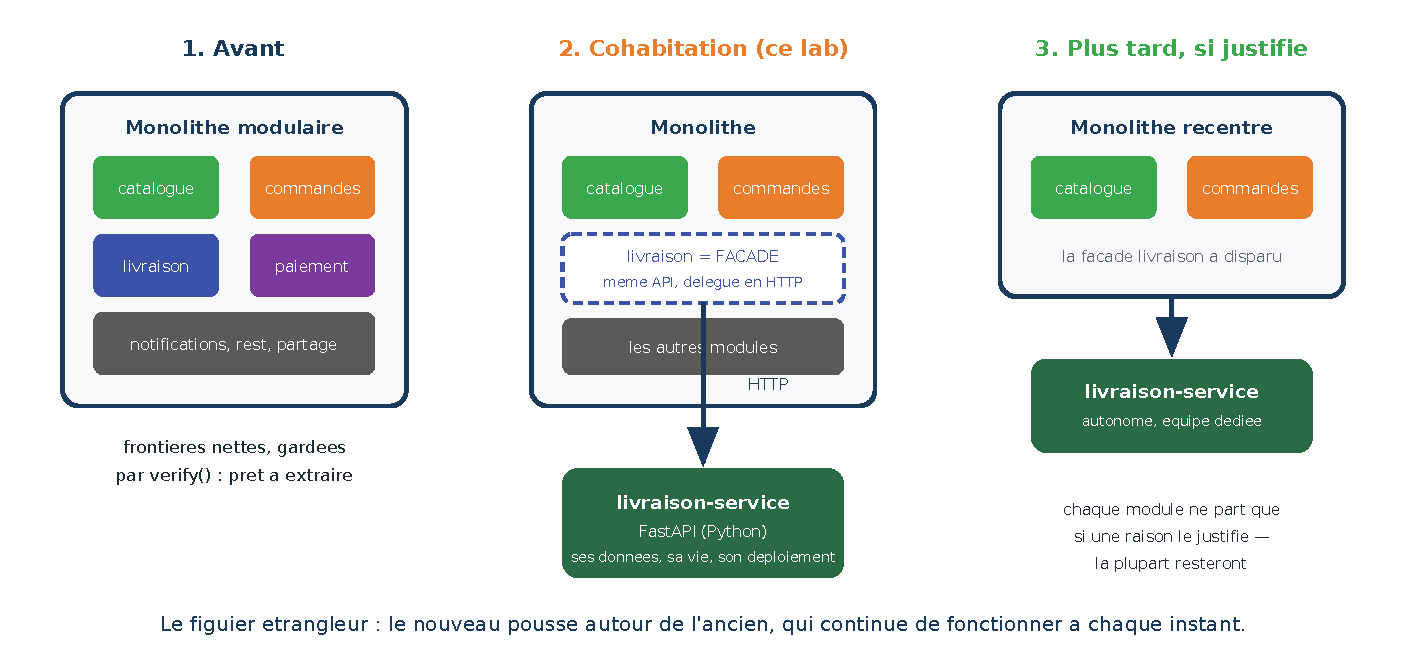
\includegraphics[width=0.64\linewidth]{figJ_strangler}
\end{frame}

\begin{frame}{Pourquoi pas le big bang ?}
{\small L'autre méthode — « on ferme, on reconstruit tout, on rouvre dans six mois » — échoue presque toujours. Trois raisons simples :}
\begin{itemize}\small
  \item \textbf{Six mois sans rien vendre} : pendant la réécriture, rien n'est livré — et les besoins, eux, continuent de changer.
  \item \textbf{Tout change le même jour} : si ça casse à l'ouverture, impossible de revenir en arrière.
  \item \textbf{On apprend trop tard} : les vrais problèmes se découvrent \emph{après} avoir tout construit.
\end{itemize}
\begin{ucadret}[Les trois règles du figuier]
{\small \textbf{1.} Le nouveau se construit \emph{à côté}, jamais \emph{à la place}. \textbf{2.} Chaque bascule peut être \emph{annulée} — chez nous : un profil Spring. \textbf{3.} L'ancien code n'est supprimé que quand \emph{plus personne ne l'appelle}.}
\end{ucadret}
\end{frame}

\begin{frame}{Le modulith paie ses dividendes}
\begin{itemize}\small
  \item Extraire \texttt{livraison} du God controller du Lab 1 aurait exigé des semaines d'archéologie. Aujourd'hui, la frontière est \textbf{déjà tracée}, l'API \textbf{déjà étroite} (\texttt{assigner}, \texttt{liberer}, \texttt{tous}), les données \textbf{déjà isolées}.
  \item La clé du lab : \texttt{AssignationLivreurs} reste en place, \textbf{même API pour \texttt{commandes}} — mais devient une \textbf{façade} qui délègue en HTTP. \texttt{commandes} ne saura jamais que livraison a déménagé.
\end{itemize}
\begin{ucadret}[À retenir — la phrase du semestre]
{\small \emph{« Monolith first, microservices when justified »} n'était pas de la prudence : c'était une \textbf{stratégie}. Le monolithe modulaire est le meilleur brouillon d'un système distribué — chaque frontière interne est une extraction en attente, qu'on ne paiera que si elle se justifie.}
\end{ucadret}
\end{frame}

% #####################################################################
\section{Traverser le réseau}

\begin{frame}{Ce que change une flèche qui sort du processus}
\centering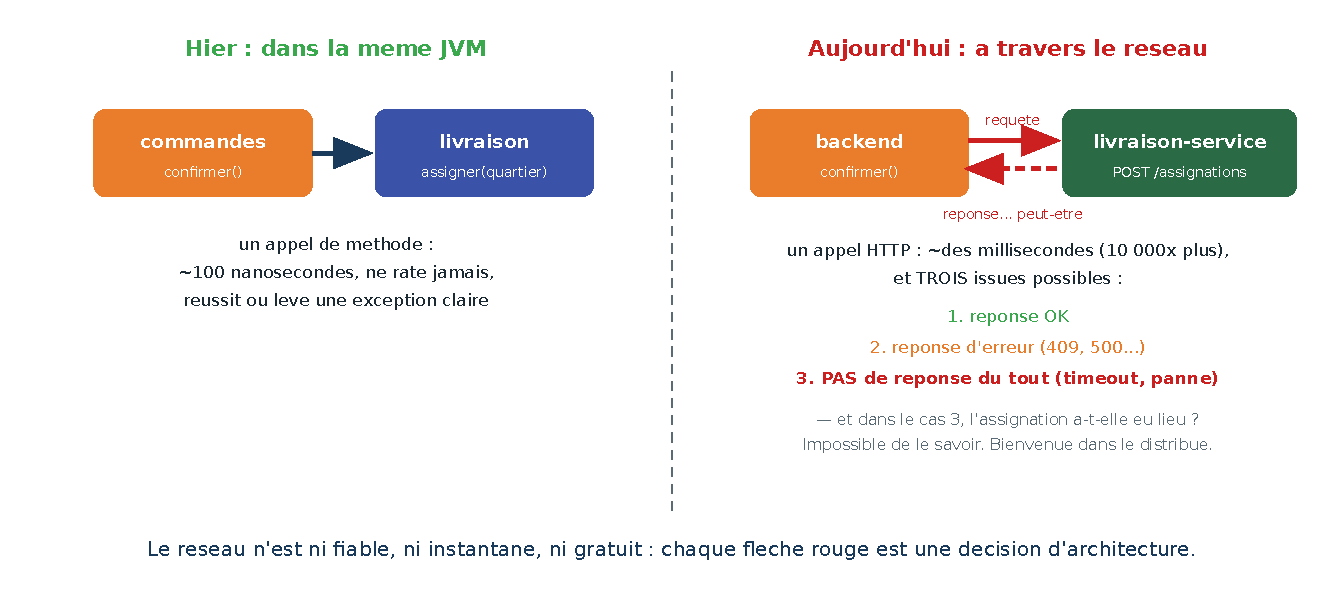
\includegraphics[width=0.76\linewidth]{figL_reseau}
\end{frame}

\begin{frame}{Le lexique du distribué}
{\small Quatre mots que ce lab installe pour de bon :}
\vskip2pt
{\small\begin{tabular}{p{0.24\linewidth}p{0.66\linewidth}}
\toprule
\textbf{Latence} & le temps aller-retour d'un appel ; \textasciitilde 100 ns en JVM, des millisecondes en HTTP — un facteur \textbf{10\,000}\\
\textbf{Timeout} & la durée maximale qu'on \emph{accepte} d'attendre avant de déclarer l'échec ; toujours \textbf{explicite}, jamais infini\\
\textbf{503} & \emph{Service Unavailable} : « je vais bien, mais quelqu'un dont je dépends ne répond pas — réessayez »\\
\textbf{Couplage temporel} & deux services qui doivent être vivants \emph{au même instant} pour coopérer — la vraie dette du synchrone\\
\bottomrule
\end{tabular}}
\vskip4pt
\begin{ucadret}[À retenir]
{\small Un timeout n'est pas un aveu d'échec : c'est une \textbf{décision d'architecte} — combien de temps la confirmation d'une commande a-t-elle le droit de retenir un client ?}
\end{ucadret}
\end{frame}

\begin{frame}{Les huit illusions du réseau}
{\small Peter Deutsch (Sun, 1994) a listé les huit croyances fausses que tout débutant du distribué paie un jour :}
\begin{columns}[t]
\begin{column}{0.48\linewidth}
{\small\begin{enumerate}
  \item Le réseau est fiable
  \item La latence est nulle
  \item La bande passante est infinie
  \item Le réseau est sûr
\end{enumerate}}
\end{column}
\begin{column}{0.48\linewidth}
{\small\begin{enumerate}\setcounter{enumi}{4}
  \item La topologie ne change pas
  \item Il y a un administrateur
  \item Transporter ne coûte rien
  \item Le réseau est homogène
\end{enumerate}}
\end{column}
\end{columns}
\vskip4pt
\begin{ucadpiege}[Celles qui nous mordent aujourd'hui]
{\small La n\textsuperscript{o}1 justifie nos timeouts et le 503 ; la n\textsuperscript{o}2, notre réflexion avant chaque extraction ; la n\textsuperscript{o}5, l'usage des \emph{noms} de services dans compose plutôt que des adresses. Les cinq autres vous attendent en entreprise.}
\end{ucadpiege}
\end{frame}

\begin{frame}{La troisième issue}
\begin{ucadpiege}[Le vrai piège du distribué]
{\small Un appel de méthode a deux issues : il réussit, ou il lève une exception. Un appel réseau en a \textbf{trois} : réponse OK, réponse d'erreur... ou \textbf{pas de réponse du tout}. Et dans ce troisième cas, impossible de savoir si l'opération a eu lieu côté serveur — le livreur a-t-il été réservé ? Vous ne le savez pas.}
\end{ucadpiege}
\begin{itemize}\small
  \item D'où les outils du distribué que ce cours introduit : \textbf{timeouts} (ne pas attendre éternellement), codes d'erreur traduits (503 quand le service est injoignable), et — au Lab 5 — l'asynchrone et l'\textbf{idempotence}.
  \item Règle d'hygiène : chaque appel réseau sortant a un \textbf{timeout explicite} et un \textbf{comportement d'échec décidé}. Jamais d'appel « optimiste ».
\end{itemize}
\begin{ucadret}[À retenir]
{\small La latence est \textbf{10\,000 fois} supérieure et l'échec devient un cas \emph{normal}. Un microservice, c'est un module qui a accepté ce contrat — c'est pour cela qu'on n'extrait pas sans raison.}
\end{ucadret}
\end{frame}

\begin{frame}[fragile]{Le contrat HTTP du nouveau service}
{\small L'API du module devient une API HTTP — traduction presque mot à mot :}
\begin{lstlisting}
POST   /assignations   {"quartier": "Medina", "restaurant_quartier": "Ouakam"}
   200 {"livreur_id": 1, "livreur_nom": "Ibrahima Ndiaye", "eta_minutes": 43}
   409 {"erreur": "Aucun livreur disponible pour le moment, ..."}
DELETE /assignations/1          # liberer le livreur 1
GET    /livreurs                # la liste (pour l'onglet Livreurs)
GET    /livreurs/1/position     # {"latitude": ..., "longitude": ...}  (carte)
\end{lstlisting}
\begin{itemize}\small
  \item Même vocabulaire, mêmes règles, mêmes messages d'erreur : le contrat métier \textbf{survit au changement de langage}. Seule la syntaxe d'appel change.
  \item Le trajet est réel : livreur $\to$ restaurant $\to$ client. Le service possède \textbf{ses} données (les livreurs) : c'est le principe \emph{database per service} — plus de table \texttt{livreur} consultée par le monolithe.
\end{itemize}
\end{frame}

% #####################################################################
\section{Conteneurs et carte}

\begin{frame}{Quatre conteneurs, un fichier}
\centering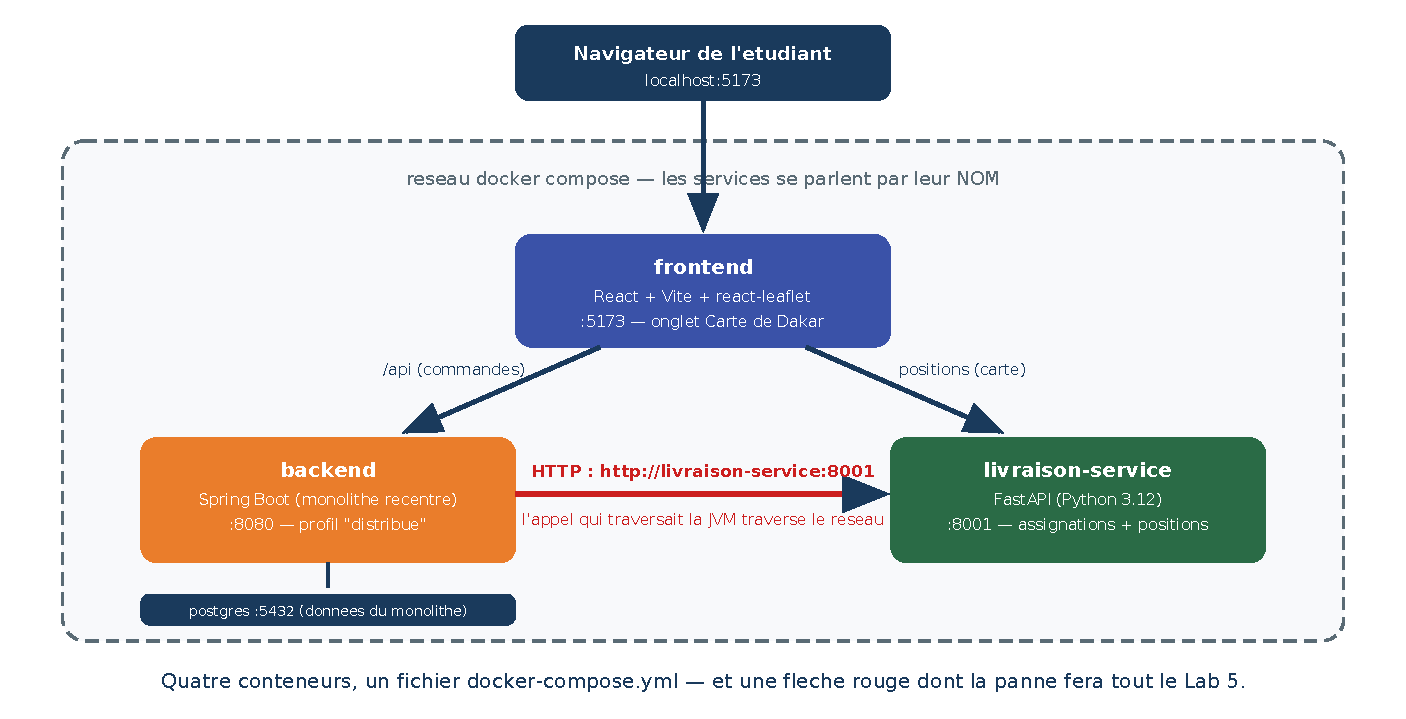
\includegraphics[width=0.70\linewidth]{figK_compose}
\end{frame}

\begin{frame}[fragile]{docker compose : l'orchestre local}
\begin{lstlisting}
services:
  postgres:            # les donnees du monolithe
    image: postgres:16
  backend:             # Spring Boot, profil "distribue"
    build: ./backend
    environment:
      - SPRING_PROFILES_ACTIVE=distribue
      - LIVRAISON_URL=http://livraison-service:8001
  livraison-service:   # FastAPI
    build: ./livraison-service
  frontend:            # React + la carte
    build: ./frontend
\end{lstlisting}
\begin{itemize}\small
  \item Sur le réseau compose, \textbf{le nom du service est son adresse} : \texttt{http://livraison-service:8001} — pas d'IP, pas de configuration réseau manuelle.
  \item Un seul geste pour tout l'orchestre : \texttt{docker compose up --build}. Et un seul pour la panne de tout à l'heure : \texttt{docker compose stop livraison-service}...
\end{itemize}
\end{frame}

\begin{frame}{La carte : Dakar en temps réel}
\begin{itemize}\small
  \item \textbf{Leaflet} + OpenStreetMap : la cartographie libre, \textbf{zéro clé API}, zéro compte — \texttt{react-leaflet} l'intègre à notre frontend en un composant.
  \item Le nouveau service expose la \textbf{position simulée} du livreur (interpolation restaurant $\to$ quartier du client au fil de l'ETA) ; le frontend l'interroge toutes les 3 secondes : le marqueur \emph{avance sur la carte de Dakar}.
  \item Ce n'est pas un gadget : c'est la \textbf{démonstration du bénéfice} — cette fonctionnalité vit entièrement dans le nouveau service, développable et déployable sans toucher au monolithe. La promesse de l'extraction, à l'écran.
\end{itemize}
\begin{ucadrec}[En pratique au lab]
{\small L'onglet « Carte » montre les restaurants (marqueurs fixes) et le livreur de la commande suivie (marqueur mobile). Quartiers, coordonnées : tout vient de \texttt{QuartiersDakar} — désormais propriété du service Python.}
\end{ucadrec}
\end{frame}

% #####################################################################
\section{Le lab}

\begin{frame}{Le chemin du Lab 4}
\centering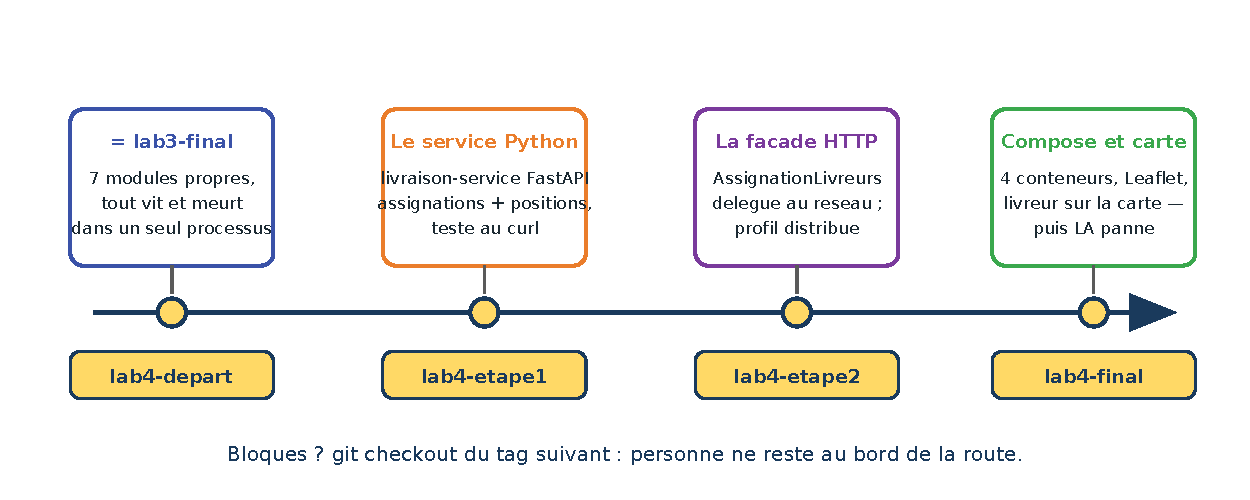
\includegraphics[width=0.80\linewidth]{figM_chemin_lab4}

{\scriptsize Point de départ : votre \texttt{lab3-final}. Et en clôture, une expérience dont le Lab 5 fera son affaire : \texttt{docker compose stop livraison-service}.}
\end{frame}

\begin{frame}{Votre mission d'aujourd'hui}
{\scriptsize\begin{tabular}{p{0.20\linewidth}p{0.72\linewidth}}
\toprule
\textbf{Rôle} & \textbf{Pilotage au Lab 4}\\
\midrule
Le Doyen & merges, tags, ADR — et l'expérience de la panne au vidéoprojecteur\\
L'Huissier & les profils Spring (monolithe / distribué) et docker compose\\
Le Rédacteur & l'onglet Carte (react-leaflet, polling des positions)\\
Le Notaire & la façade HTTP : \texttt{AdaptateurLivraisonHttp} (RestClient, timeouts)\\
L'Appariteur & le service FastAPI : assignations, positions, données livreurs\\
\bottomrule
\end{tabular}}
\vskip4pt
\begin{ucadrec}[Le livrable individuel de la séance]
{\small L'\textbf{Architecte du jour} signe l'\textbf{ADR n\textsuperscript{o}4 : « Pourquoi extraire Livraison — et pourquoi pas les autres ? »} — le premier ADR qui doit défendre des \emph{non-décisions}.}
\end{ucadrec}
\end{frame}

\begin{frame}{L'essentiel de la séance}
\begin{ucadret}[À retenir]
{\footnotesize
\begin{itemize}
  \item On extrait un module pour \textbf{trois raisons} : technologie, déploiement indépendant, dimensionnement — jamais pour la mode. La charge de la preuve incombe à l'extraction.
  \item Le \textbf{Strangler Fig} : le nouveau pousse autour de l'ancien, l'application fonctionne à chaque instant — et le modulith avait déjà tracé la frontière.
  \item Un appel réseau a \textbf{trois issues}, coûte 10\,000 fois plus cher, et exige timeout + comportement d'échec explicites.
  \item \textbf{docker compose} : le nom du service est son adresse ; quatre conteneurs, un fichier, un geste.
\end{itemize}}
\end{ucadret}
\begin{ucadfront}[La question qui ouvre la séance 5]
{\footnotesize En fin de lab, nous tuerons \texttt{livraison-service}... et la confirmation de commande mourra avec lui. Un service peut-il tomber \emph{sans entraîner les autres} ? Réponse au Lab 5 : l'asynchrone — RabbitMQ, et des événements qui attendent patiemment le retour des absents.}
\end{ucadfront}
\end{frame}

\end{document}
